\documentclass{report}

\usepackage{a4}
\usepackage{psfig}
\usepackage{ebnf}
\usepackage{booster}


\bibliographystyle{mybibsty}

\begin{document}

%%%%%%%%%%%%%%%%%%%%%%%%%%%%%%%%%%%%%%%%%%%%%%%%%%%%%%%%%%%%%%%%%%%%%%%%%%%%%%
%Fill in the following lines:                                                %
%%%%%%%%%%%%%%%%%%%%%%%%%%%%%%%%%%%%%%%%%%%%%%%%%%%%%%%%%%%%%%%%%%%%%%%%%%%%%%
\newcommand{\cptitle}{The Booster Language\\Syntax and Static Semantics}
\newcommand{\cpauthors}{
\begin{tabular}{ccc}
Leo Breebaart  & $\quad$ & Paul Dechering\\
Arnaud Poelman & 	 & Joachim Trescher\\
Hans de Vreught& 	 & Henk Sips\\
\end{tabular}}
\newcommand{\cpyear}{95}
\newcommand{\cpnumber}{2}
\newcommand{\cpissn}{1382-5224}
%%%%%%%%%%%%%%%%%%%%%%%%%%%%%%%%%%%%%%%%%%%%%%%%%%%%%%%%%%%%%%%%%%%%%%%%%%%%%%

\begin{titlepage}
\thispagestyle{empty}
\begin{center}
\bfseries
\Large
Delft University of Technology \\
Computational Physics Report Series \\[2\baselineskip]
{\huge \cptitle} \\[\baselineskip]
{\large\normalfont \cpauthors} \\[2\baselineskip]
report number  CP-\cpyear-\cpnumber \\
\vfill
\begin{figure}[htbp]
  \begin{center}
    \mbox{
\psfig{file=CP.eps,width=7.5cm,height=5.5cm}}
  \end{center}
\end{figure}
\vfill
ISSN \cpissn
\end{center}
\pagebreak
\thispagestyle{empty}
\noindent
\begin{tabular}{l}
Published and produced by: \\
Computational Physics Section \\
Faculty of Applied Physics \\
Delft University of Technology \\
Lorentzweg 1 \\
2628 CJ  Delft \\
The Netherlands \\
 \\
Information about Computational Physics Report Series: \\
\textsf{reports@cp.tn.tudelft.nl} \\
 \\
Information about Computational Physics Section: \\
\textsf{http://www.cp.tn.tudelft.nl/} \\
\end{tabular}
\vfill
\noindent
\copyright\ 19\cpyear\ Computational Physics Section, Faculty of Applied
Physics, Delft University of Technology. All rights reserved. No part of this
series may be reproduced in any form or by any means without prior written
permission of the publisher.
\end{titlepage}


\chapter*{Booster in Perspective}

  This series of technical reports account for the detailed description of
the \Booster\ language and its semantics.

The \Booster\ project has a long history. The project started off in 1988 and
had as goal the development of a high level language for scientific
programming on parallel computers, which would pair expressiveness with
efficiency of execution.

The first concepts of the language have been presented in 1989
\cite{Paalvast89} \cite{Paalvast89a}. The major features of \Booster,
such as the View concept and the separation of algorithm description
and machine mapping were introduced.

At the same time, the first thoughts on how to translate such a
language were developed. It was felt that a properly defined semantic
system was required to be able to translate and optimize programs in
such a high-level language. After some investigations it was decided
to take a calculus-based approach, since this would enable us to
define transformations in the form of rewriting expressions. This
approach is also followed in translating functional languages with the
$\lambda$-calculus as basic semantic formalism \cite{Jones87}.
However, the $\lambda$-calculus is not a very adequate vehicle for
expressing optimizations \cite{Plasmeijer93} and certainly not for
array based operations.  Other formalisms, such as the Bird-Meertens
formalism \cite{Bird89} which is essentially list-based, had the same
problems.

Hence it was decided to develop an array based calculus named {\sl
V}-cal.  A first outline of such a calculus was given in
\cite{vanGemund89}. In \cite{Paalvast90} it was shown how this
calculus could be used in translating \Booster\ and in \cite{Paalvast91}
it was shown that SPMD programs could automatically be derived from
data decomposition descriptions in any similar language.

Based on these developments a full definition of the \Booster\ language
and {\sl V}-cal were given in Paalvast's PhD thesis
\cite{Paalvast92}. He also showed how \Booster\ programs could be
transformed into {\sl V}-cal expressions. Other papers giving global
descriptions of the \Booster\ language are \cite{Paalvast91a}, and
\cite{deJong92}.

A third important decision in the \Booster\ project was to use
rule-based translation technology for translating and optimizing
\Booster\ programs, an approach inspired by \cite{Wang91}. The rationale
for this approach was that rule-based compilation would enable easy
experimentation with several transformation schemes and give a
flexible tool for experimentation. A rule-based translation system was
developed \cite{Breebaart92} \cite{Breebaart92a} and used as a first
translation system.

With all three things in place: the \Booster\ language definition,
{\sl V}-cal, and the rule-based translator efforts began in 1993 to
make a full compiler for the language. During that time it was found
that the automatic translation of \Booster\ constructs to {\sl V}-cal
expressions gave rise to difficulties. In part this was due to the
expressive power of the \Booster\ language itself, but also missing
abstractions in {\sl V}-cal caused technical problems. 

A possible solution could have been to define arbitrary restrictions
for the \Booster language, but we did not want to end with complicated
and inelegant static semantics, like found in for instance Fortran 90.
Instead a redesign of both language and calculus has taken place in
1994.  \Booster\ has been restricted somewhat, especially regarding
data dependent views. On the other hand, some features have been
added, such as to allow function calls in view expressions and
function recursion. \Booster's denotational semantics have been defined
such that any \Booster\ program can now mechanically be translated
into {\sl V-cal} expressions.  A global outline of the new approach
can be found in \cite{Trescher94}.

In perspective, \Booster\ has been one of the early data parallel
languages.  Other early efforts were directed towards extending
existing languages like C* \cite{Quinn89}, Kali \cite{Koelbel91}, Id
nouveau \cite{Rogers89}, and Fortran \cite{Gerndt89}
\cite{Callahan88}. Later on these developments found their way in the
definition of High Performance Fortran \cite{HPFF93} in which most of
these research groups participated.

\vspace{2\baselineskip}

\noindent Henk Sips \hfill{\today}


\chapter*{Preface}

  \Booster\ is an experimental data parallel language. Its most
important features are super scalar statements, the view concept, and
annotations.

Super scalar statements make \Booster\ a data parallel language. The
view concept allows concise descriptions of intricate algorithms by
providing the facilities to construct, compose, and compute index
sets. Annotations provide a flexible means to specify data
distributions.

This report is intended to serve as a reference for programmers and
implementors and is, therefore, kept concise. More information on
\Booster\ can be found in the companion reports ``Booster?!? Never
heard of it - A Tutorial'' \cite{Dechering95} and ``The Denotational
Semantics of Booster'' \cite{Dechering95a}.

\Booster\ is an experimental language and we expect it to evolve with
experience. The most recent version of the \Booster\ language
definition can be found in
\verb'ftp://ftp.cp.tn.tudelft.nl/~/pub/cp/publications/1995'.

\section*{Booster in Perspective}

The \Booster\ project has a long history. The project started off in
1988 and with as goal the development of a high level language for
scientific programming on parallel computers, which would pair
expressiveness with efficiency of execution.

The first concepts of the language have been presented in 1989
\cite{Paalvast89} \cite{Paalvast89a}. The major features of \Booster,
such as the View concept and the separation of algorithm description
and machine mapping were introduced.

At the same time, the first thoughts on how to translate such a
language were developed. It was felt that a properly defined semantic
system was required to be able to translate and optimize programs in
such a high-level language. After some investigations it was decided
to take a calculus-based approach, since this would enable us to
define transformations in the form of rewriting expressions. This
approach is also followed in translating functional languages with the
$\lambda$-calculus as basic semantic formalism \cite{Jones87}.
However, the $\lambda$-calculus is not a very adequate vehicle for
expressing optimizations \cite{Plasmeijer93} and certainly not for
array based operations.  Other formalisms, such as the Bird-Meertens
formalism \cite{Bird89} which is essentially list-based, have the same
problems.

Hence it was decided to develop an array based calculus named {\sl
V}-cal.  A first outline of such a calculus was given in
\cite{vanGemund89}. In \cite{Paalvast90} it was shown how this
calculus could be used in translating \Booster\ and in \cite{Paalvast91}
it was shown that SPMD programs could automatically be derived from
data decomposition descriptions in any similar language.

Based on these developments a definition of the \Booster\ language and
{\sl V}-cal were given in Paalvast's PhD thesis
\cite{Paalvast92}. He also showed how \Booster\ programs could be
transformed into {\sl V}-cal expressions. Other papers giving global
descriptions of the \Booster\ language are \cite{Paalvast91a}, and
\cite{deJong92}.

A third important decision in the \Booster\ project was to use
rule-based translation technology for translating and optimizing
\Booster\ programs, an approach inspired by \cite{Wang91}. The rationale
for this approach was that rule-based compilation would enable easy
experimentation with several transformation schemes and give a
flexible tool for experimentation. To that aim, a rule-based
translation system was developed \cite{Breebaart92}
\cite{Breebaart92a}.

With all three things in place: the \Booster\ language definition,
{\sl V}-cal, and the rule-based translator efforts began in 1993 to
make a full compiler for the language. During that time it was found
that the automatic translation of \Booster\ constructs to {\sl V}-cal
expressions gave rise to difficulties. In part this was due to the
expressive power of the \Booster\ language itself, but also missing
abstractions in {\sl V}-cal caused technical problems. 

A possible solution could have been to define case-baesd restrictions
for the \Booster\ language, but we did not want to end with complicated
and inelegant static semantics, like found in for instance Fortran 90.
Instead a redesign of both language and calculus has taken place in
1994.  \Booster\ has been restricted somewhat, especially regarding
data dependent views. On the other hand, some features have been
added, such as to allow function calls in view expressions and
function recursion. \Booster's denotational semantics have been
defined such that any \Booster\ program can now mechanically be
translated into {\sl V-cal} expressions.  A global outline of the new
approach can be found in \cite{Trescher94}.

In perspective, \Booster\ has been one of the early data parallel
languages.  Other early efforts were directed towards extending
existing languages like C* \cite{Quinn89}, Kali \cite{Koelbel91}, Id
nouveau \cite{Rogers89}, and Fortran \cite{Gerndt89}
\cite{Callahan88}. Later on these developments found their way in the
definition of High Performance Fortran \cite{HPFF93} in which most of
these research groups participated.


\chapter{The Grammar}\label{BoosterGrammar}

  % Written by:
% * Paul Dechering
% * Arnaud Poelman
% * Joachim Trescher
% * Hans de Vreught

We define the syntax of \Booster\ using an extended {\small BNF}. The
extensions have the following meaning:

\begin{tabular}{ll}
\\
{\em EBNF Construct} & {\em Meaning}\\
\\
\terminal{$\alpha$} & $\alpha$ is a terminal symbol\\
\optional{$\alpha$} & zero or one $\alpha$ \\
\compound{$\alpha$}  & $\alpha$ is a syntactical unit\\
$\alpha$\separation{$\beta$} & a non empty sequence of $\alpha$'s
separated by $\beta$'s \\
\any{$\alpha$} & an arbitrary number of $\alpha$'s\\
\iteration{$\alpha$} & one or more $\alpha$'s\\
$\alpha \beta$ & first $\alpha$ then $\beta$\\
$\alpha$\alternative $\beta$ & either $\alpha$ or $\beta$
\end{tabular}

\section{Modules}

\begin{production}
\NT{Booster}
   & \rewrite & \NT{DefinitionModule} \\
   & \alternative & \NT{ImplementationModule} \\
   & \alternative & \NT{AnnotationModule} \\
   & \point \\
\NT{DefinitionModule}
   & \rewrite & \NT{DefinitionHeader} \NT{DefinitionBody} \\
   & \point \\
\NT{DefinitionHeader}
   & \rewrite & \T{DEFINITION} \T{MODULE} \TC{Identifier} \T{;} \\
   & \point \\
\NT{DefinitionBody}
   & \rewrite & \any{\NT{DefinitionUnit}} \T{END} \TC{Identifier} \T{.} \\
   & \point \\
\NT{ImplementationModule}
   & \rewrite & \NT{ImplementationHeader} \NT{ImplementationBody} \\
   & \point \\
\NT{ImplementationHeader}
   & \rewrite & \optional{\T{IMPLEMENTATION}} \T{MODULE} \TC{Identifier} \T{;} \\
   & \point \\
\NT{ImplementationBody}
   & \rewrite & \any{\NT{ImplementationUnit}} \optional{\T{BEGIN} \NT{StatementList}} \\
   & & \tab \T{END} \TC{Identifier} \T{.} \\
   & \point \\
\NT{AnnotationModule} & \rewrite & \NT{AnnotationHeader} \NT{AnnotationBody} \\
   & \point \\
\NT{AnnotationHeader} & \rewrite & \T{ANNOTATION} \T{MODULE} \TC{Identifier} \T{;} \\
   & \point \\
\NT{AnnotationBody} & \rewrite & \any{\NT{AnnotationUnit}}
                      \optional{\T{BEGIN} \NT{AnnotationList}}\\
   & & \tab \T{END} \TC{Identifier} \T{.} \\
   & \point \\
\end{production}

\section{Units}

\begin{production}
\NT{DefinitionUnit}
   & \rewrite & \NT{ImportDefinition} \\
   & \alternative & \NT{ConstDefinition} \\
   & \alternative & \NT{TypeDefinition} \\
   & \alternative & \NT{VarDeclaration} \\
   & \alternative & \NT{ProcedureHeader} \\
   & \alternative & \NT{FunctionHeader} \\
   & \point \\
\NT{ImplementationUnit}
   & \rewrite & \NT{ImportDefinition} \\
   & \alternative & \NT{ConstDefinition} \\
   & \alternative & \NT{TypeDefinition} \\
   & \alternative & \NT{VarDeclaration} \\
   & \alternative & \NT{Procedure} \\
   & \alternative & \NT{Function} \\
   & \point \\
\NT{AnnotationUnit}
   & \rewrite & \NT{ImportDefinition}\\
   & \alternative & \NT{MachineDeclaration}\\
   & \point \\
\NT{ImportDefinition}
   & \rewrite & \optional{\T{FROM} \TC{Identifier}} \T{IMPORT}
     \compound{\TC{Identifier} \separation \T{,}} \T{;} \\ 
   & \point \\ 
\NT{ConstDefinition}
   & \rewrite &  \T{CONST} \NT{ConstList} \T{END} \T{;} \\
   & \point \\
\NT{TypeDefinition}
   & \rewrite &  \T{TYPE} \NT{TypeList} \T{END} \T{;} \\
   & \point \\
\NT{VarDeclaration}
   & \rewrite & \T{VAR} \NT{DeclarationList} \T{END} \T{;} \\
   & \point \\
\NT{MachineDeclaration}
   & \rewrite & \T{MACHINE} \NT{DeclarationList} \T{END} \T{;} \\
   & \point \\
\NT{Procedure}
   & \rewrite & \NT{ProcedureHeader} \NT{Body} \\
   & \point \\
\NT{ProcedureHeader}
   & \rewrite & \optional{\T{EXTERN}} \T{PROCEDURE} \TC{Identifier}\\
   &          & \tab  \T{(} \optional{\NT{ArgumentList}} \T{)} \T{;} \\  
   & \point \\
\NT{Function}
   & \rewrite & \NT{FunctionHeader} \NT{Body} \\
   & \point \\
\NT{FunctionHeader}
   & \rewrite & \optional{\T{EXTERN}} \T{FUNCTION} \TC{Identifier}
                  \T{(}\optional{\NT{ArgumentList}}\T{)} \\ 
   &  & \tab \T{RESULT} \NT{SingleDeclaration} \T{;} \\
   & \point \\
\NT{Body}
   & \rewrite & \optional{\NT{VarDeclaration}} \T{BEGIN}
   \NT{StatementList}\\
   &  & \tab \T{END} \TC{Identifier} \T{;} \\ 
   & \point \\
\end{production}

\section{Declarations}

\begin{production}
\NT{ConstList}
   & \rewrite & \optional{\TC{Identifier} \T{=} \NT{Expression}} \separation\ \T{;} \\
   & \point \\
\NT{TypeList}
   & \rewrite & \optional{\TC{Identifier} \T{=} \NT{Type}} \separation\ \T{;} \\
   & \point \\
\NT{DeclarationList}
   & \rewrite & \optional{\compound{\TC{Identifier} \separation\ \T{,}} \T{:} \NT{Type}} \separation\ \T{;} \\
   & \point \\
\NT{SingleDeclaration}
   & \rewrite & \TC{Identifier} \T{:} \NT{Type} \\
   & \point \\
\NT{ArgumentList}
   & \rewrite & \NT{Argument} \separation\ \T{;} \\
   & \point \\
\NT{Argument}
   & \rewrite & \NT{FlowType} \compound{\TC{Identifier} \separation\ \T{,}} \T{:} \NT{Type} \\
   & \point \\
\NT{FlowType}
   & \rewrite & \T{IN} \alternative\ \T{OUT} \alternative\ \T{INOUT} \\
   & \point \\
\NT{Type}
   & \rewrite & \TC{Identifier} \\
   & \alternative & \NT{TypeConstructor} \\
   & \point \\
\NT{TypeConstructor}
   & \rewrite & \NT{Kind} \verb*"{"* \NT{CardinalityList} \verb*"}" \T{OF}
                \NT{Type} \\ 
   & \point \\
\NT{Kind}
   & \rewrite & \T{SHAPE}\\
   & \alternative & \T{VIEW}\\
   & \point\\
\NT{CardinalityList}
   & \rewrite & \NT{Cardinality} \separation\ \T{\#} \\
   & \point \\
\NT{Cardinality}
   & \rewrite & \T{CONST} \TC{Identifier} \\
   & \alternative & \optional{\TC{Identifier} \T{:}} \NT{Expression} \\
   & \alternative & \T{*} \\
   & \point \\
\end{production}

\section{Flow of Control}

\begin{production}
\NT{AnnotationList}
   & \rewrite & \optional{\NT{AnnotationStatement}} \separation\ \T{;} \\
   & \point \\
\NT{StatementList}
   & \rewrite & \optional{\NT{Statement}} \separation\ \T{;} \\
   & \point \\
\NT{Statement}
   & \rewrite & \NT{ControlFlowStatement} \\
   & \alternative & \NT{ViewStatement} \\
   & \alternative & \NT{ContentStatement} \\
   & \alternative & \NT{ProcedureCall} \\
   & \point \\
\NT{ControlFlowStatement}
   & \rewrite & \NT{WhileStatement} \\
   & \alternative & \NT{IterStatement} \\
   & \alternative & \NT{IfStatement} \\
   & \point \\
\NT{WhileStatement}
   & \rewrite & \T{WHILE} \NT{Expression} \T{DO} \NT{StatementList} \T{END} \\
   & \point \\
\NT{IterStatement}
   & \rewrite & \T{ITER} \NT{Expression} \T{TIMES} \NT{StatementList} \T{END} \\
   & \alternative & \T{ITER} \TC{Identifier} \T{OVER} \NT{Expression} \\
   & & \tab \T{DO} \NT{StatementList} \T{END} \\
   & \point \\
\NT{IfStatement}
   & \rewrite & \T{IF} \NT{Expression} \T{THEN} \NT{StatementList} \optional{\NT{ElsePart}} \T{END} \\
   & \point \\
\NT{ElsePart}
   & \rewrite & \T{ELSE} \NT{StatementList} \\
   & \alternative & \T{ELSEIF} \NT{Expression} \T{THEN} \NT{StatementList} \optional{\NT{ElsePart}} \\
   & \point \\
\end{production}

\section{Statements}

\begin{production}
\NT{AnnotationStatement}
   & \rewrite & \NT{AnnotationDesignator} \T{$\mathtt{<-}$} \NT{Structure} \\
   & \point \\
\NT{AnnotationDesignator} 
   & \rewrite & \NT{QualIdent} \optional{\T{\{} \NT{CardinalityList} \T{\}}} \\
   & \point \\
\NT{ViewStatement}
   & \rewrite & \NT{ViewDesignator} \T{$<-$} \NT{Structure} \\
   & \point \\
\NT{ViewDesignator} 
   & \rewrite & \NT{QualIdent} \optional{\T{\{} \NT{CardinalityList} \T{\}}} \\
   & \point \\
\NT{ContentStatement}
   & \rewrite & \NT{ContentDesignator} \NT{Assignment} \NT{Expression} \\
   & \point \\
\NT{Assignment}
   & \rewrite & \T{:=} \\
   & \alternative & \T{||=} \\
   & \point \\
\NT{ContentDesignator}
   & \rewrite & \NT{Structure} \\
   & \point \\
\NT{SelectorList}
   & \rewrite & \NT{Selector} \separation\ \T{,} \\
   & \point \\
\NT{Selector}
   & \rewrite & \optional{\TC{Identifier} \T{:}} \NT{Expression} \\
   & \point \\
\NT{ProcedureCall}
   & \rewrite & \NT{QualIdent} \T{(} \optional{\NT{ExpressionList}} \T{)}  \\
   & \point \\
\end{production}

\section{Expressions}

\begin{production}
\NT{Expression}
   & \rewrite & \NT{Expression} \TC{RelOp} \NT{ArithmeticExpression} \\
   & \alternative & \NT{ArithmeticExpression} \\
   & \point \\
\NT{ArithmeticExpression}
   & \rewrite & \NT{ArithmeticExpression} \TC{AddOp} \NT{Term} \\
   & \alternative & \NT{Term} \\
   & \point \\
\NT{Term}
   & \rewrite & \NT{Term} \TC{MulOp} \NT{Factor} \\
   & \alternative & \NT{Factor} \\
   & \point \\
\NT{Factor}
   & \rewrite & \optional{\TC{UnOp}} \T{(} \compound{\NT{Expression} \separation \T{,}} \T{)}  \\
   & \alternative &  \optional{\TC{UnOp}} \T{\{} \NT{ExpressionList} \T{\}} \\
   & \alternative & \optional{\TC{UnOp}} \NT{Structure} \\
   & \alternative & \optional{\TC{UnOp}} \TC{Number} \\
   & \alternative & \optional{\TC{UnOp}} \T{\$} \\
   & \alternative & \TC{StringLiteral} \\
   & \alternative & \T{\_} \\
   & \point \\
\NT{ExpressionList}
   & \rewrite & \NT{Expression} \separation\ \T{,} \\
   & \point \\
\NT{Structure}
   & \rewrite & \NT{FunctionCall} \\
   & \alternative & \NT{Designator} \\
   & \point \\
\NT{FunctionCall}
   & \rewrite & \optional{\TC{Identifier} \T{.}} \TC{Identifier} \T{(}
   \optional{\NT{ExpressionList}} \T{)}\\
   & & \tab  \optional{\T{[} \NT{SelectorList} \T{]}} \\ 
   & \point \\
\NT{Designator} 
   & \rewrite & \optional{\TC{Identifier} \T{.}} \TC{Identifier} \optional{\T{[} \NT{SelectorList \T{]}}} \\
   & \point \\
\end{production}

\section{Tokens}

\begin{production}
\TC{RelOp}
   & \rewrite & \T{>} \alternative\ \T{>=} \alternative\ \T{<>} \alternative\ \T{=} \alternative\ \T{<=} \alternative\ \T{<} \alternative\ \T{|} \\
   & \point \\
\TC{AddOp}
   & \rewrite & \T{OR} \alternative\ \T{+} \alternative\ \T{-} \alternative\ \T{\&} \\
   & \point \\
\TC{MulOp}
   & \rewrite & \T{AND} \alternative\ \T{DIV} \alternative\ \T{MOD} \alternative\ \T{*} \alternative\ \T{/} \alternative\ \T{..} \\
   & \point \\
\TC{UnOp}
   & \rewrite & \T{NOT} \alternative\ \T{+} \alternative\ \T{-} \alternative\ \T{$\backslash$} \\
   & \point \\
\TC{Identifier}
   & \rewrite & \TC{Letter} \any{\compound{\TC{Letter} \alternative\ \TC{Digit}}} \\
   & \point \\
\TC{Letter}
   & \rewrite & \T{A} \class\ \T{Z} \alternative\ \T{a} \class\ \T{z} \\
   & \point \\
\TC{Number}
   & \rewrite & \iteration{\TC{Digit}} \optional{\T{.} \iteration{\TC{Digit}}} \optional{\T{E} \optional{\T{+} \alternative\ \T{-}} \iteration{\TC{Digit}}} \\
   & \point \\
\TC{Digit}
   & \rewrite & \T{0} \class\ \T{9} \\
   & \point \\
\TC{StringLiteral}
   & \rewrite & \T{'} \any{\compound{\TC{Character} \alternative\ \TC{EscapedCharacter}}} \T{'} \\
   & \point \\
\TC{EscapedCharacter}
   & \rewrite & \T{$\backslash$b} \alternative\ \T{$\backslash$f} \alternative\ \T{$\backslash$n} \alternative\ \T{$\backslash$r} \alternative\ \T{$\backslash$t} \alternative\ \T{$\backslash$'} \alternative\ \T{$\backslash\backslash$} \\
   & \alternative & \T{$\backslash$} \TC{Digit} \optional{\TC{Digit}
   \optional{\TC{Digit}}} \\
   & \point \\
\TC{Character}
   & \rewrite & $\Sigma\setminus$\compound{\T{$\backslash$} \alternative\ \T{'}} \\
   & \point \\
\end{production}

\noindent
$\Sigma$ contains all printable ASCII characters \T{ } \class\ \T{\~{}}.

\section{White Space}

White space outside string literals may be used to separate tokens and is no
part of the language. It should be filtered out before parsing starts under
the condition that separated tokens remain separated. Beside space, tab,
linefeed, carriage return, and formfeed comments also count as white space.
There are two types of comments:
\begin{itemize}
\item A comment starts with \T{//} and ends at the end of the line. This is a
	single line comment.
\item A comment starts with \T{/*} and ends with \T{*/}. These comments may
	be nested.
\end{itemize}


\chapter{The Static Semantics}

  \section{Definitions}

\Booster\ programs specify computations that act on components
called {\em locations}. {\em Variables\/} are bounded sets of
locations that represent a value determined by the variable's {\em
type}. If a value {\sc v} can be represented by a variable of type
{\sc t}, then we say the value is a {\em member} of {\sc t}, and {\sc
t} {\em contains} the value {\sc v}.

The {\em form} of a variable is the sequence of its length in each
dimension. The form of a zero dimensional variable (i.e.\ scalar) is
the empty sequence.

An {\em expression\/} specifies a computation that produces a value, a
variable, or an enumeration of natural values called a {\em
selection}. Expressions that produce variables are called {\em
designators}. A designator can denote either a variable or the value
of that variable, depending on the context. Expressions that produce
selections are called {\em set expressions}. Expressions whose values
can be determined statically are called {\em constant expressions}.

\subsection*{Notational conventions}

For the rest of this document we adopt the following notational
conventions: 

\begin{itemize}

\item let \NT{NT} be a nonterminal of the \Booster\ grammar, the term
\Language{\NT{NT}} denotes the language defined by the production
rules of the \Booster\ grammar and the start symbol \NT{NT}.

\item For the representation of \Booster\ program fragments we will use
constructs of the extended BNF defined in Chapter \ref{BoosterGrammar}
in an obvious way. Identifiers surrounded by \verb'<' and \verb'>'
denote the language construct suggested by the Booster grammar. For
instance, in the program fragment

\begin{frag}
{[}IMPLEMENTATION{]} MODULE <Id$_{\tt 1}$>;\\
\> <ImplementationUnits>\\
\> [BEGIN <StatementList>]\\
END <Id$_{\tt 2}$>.
\end{frag}

\noindent the parts between brackets are optional. Furthermore, {\small
\tt <Id$_{\tt 1}$>} and {\small \tt <Id$_{\tt 2}$>} are elements of
\Language{\TC{Identifier}}, {\small \tt <ImplementationUnits>} $\in$
\any{\Language{\NT{ImplementationUnit}}}, and {\small \tt
<StatementList>} $\in$ \Language{\NT{StatementList}}.

\end{itemize}

\subsection*{Representation}

The representation of terminal symbols in terms of characters is
defined using the ASCII set. Symbols are identifiers, numbers,
strings, operators, and delimiters. The following lexical rules must
be observed: Blanks and line breaks must not occur within symbols,
they are ignored unless they are essential to separate two consecutive
symbols. Capital and lower-case letters are considered as distinct.

\begin{description}

\item[Identifiers] are symbols (represented by a sequence of letters
and digits whose first character is a letter) declared as a name for a
type, variable, procedure etc.

\item[Numbers] are natural, integer, real, or complex
constants. The type of a natural or  integer constant is the minimal
type to which the value belongs. A real number always contains a
decimal point; optionally it may also contain a decimal scale factor.
The letter ``E'' means ``times ten to the power of.'' A complex number
is represented by a tuple $(r_1, r_2)$ of two real numbers where $r_1$
represents the real part and $r_2$ represents the imaginary part of
the complex number.

\item[Strings] are sequences of characters enclosed in single (')
quote marks.

\item[Operators and delimiters] are the special symbols listed
below. The reserved words consist exclusively of capital letters and
must not be declared as identifiers.

{\small \tt
\begin{tabular}{lllll}
\verb'+' & \verb':='  & AND            & IN        & THEN\\
\verb'-' & \verb'*'   & BEGIN          & INOUT     & TIMES\\
\verb'=' & \verb'<>'  & CONST          & ITER      & TYPE\\
\verb'>=' & \verb'<=' & DEFINITION     & MOD       & VAR\\
\verb'#' & \verb'&'   & DIV            & MODULE    & VIEW\\
\verb'<-' & \verb"//" & DO             & MACHINE   & WHILE\\    
\verb'|' & \verb"'"   & ELSE           & NOT\\	   
\verb'/' & \verb'..'  & ELSIF          & OF\\
\verb',' & \verb'.'   & END            & OR\\
\verb'\' & \verb';'   & EXTERN	       & OUT\\
\verb'_' & \verb':'   & FROM           & OVER\\
\verb'(' & \verb')'   & FUNCTION       & PROCEDURE\\
\verb'[' & \verb']'   & IF             & PROCESSORS\\
\verb'{' & \verb'}'   & IMPLEMENTATION & RESULT\\
\verb'/*' & \verb'*/' & IMPORT         & SHAPE\\
\end{tabular}}

\end{description}

\subsection*{Scope rules}

Every identifier occuring in a program must be introduced by a
declaration or import, unless it is a predeclared
identifier. Declarations also specify certain permanent properties of
an identifier, such as whether it is a constant, a type, a variable
(and its type), or a procedure.  The identifier is used to refer to
the associated entity.

The scope of an identifier is the block (module, procedure, function,
or statement) to which the declaration belongs and to which the
identifier is local. Scopes can be nested. The meaning of an
identifier is determined by the smallest enclosing scope in which the
identifier is declared. Entities referred to by declared identifiers
are called {\em visible}.

\subsection*{Name spaces}

Each scope $S$ consists of three {\em name spaces}:

\begin{enumerate}

\item The set $\TypeDefSet \subseteq \{(A, T) | A \in
\Language{\TC{Identifier}} \mbox{ and } T \in \Language{\NT{Type}}\}$
represents the set of user defined type definitions; i.e. $(A,T) \in
\TypeDefSet$ iff in S a type definition $A\ \T{=}\ T$ is visible. The
set $\TypeDefSet$ must define a function. An identifier $A$ such that
there exists a type $T$ and $(A, T) \in {\cal T}$ is called a {\em
declared} type.

\item The set of function and procedure identifiers ${\cal F}$ is
defined by the set of function and procedure declarations visible
within $S$.  An identifier in ${\cal F}$ is called a {\em declared}
procedure or function.

\item The set ${\cal D}$ of variable, view, and constant identifiers
defined by variable and constant declarations, or the variable
bindings of a selector visible within $S$. An identifier in ${\cal D}$
is called a {\em declared} variable, view or constant.

\end{enumerate}

\subsection*{Errors}

A {\em static error} is an error that a language implementation must
detect and report before program execution. Violations of the language
definition are static errors unless they are explicitely classified as
runtime errors.

A {\em checked runtime error} is an error that a language
implementation must detect and report. The method for reporting such
errors is implementation-dependent. For reasons of efficiency a
language implementation should provide a compiler option that
suppresses checking and reporting of runtime errors. The occurrence of
an {\em unchecked runtime error} may cause the subsequent behaviour of
a computation to be arbitrary.


  % Written by:
% * Joachim Trescher
% * Hans de Vreught

\section{Types}

In \Booster\ a {\em type} is specified by an expression in
\Language{\NT{Type}} and represents a set of values.  \Booster\ uses
structural type equivalence: two types are the same if their
definitions become the same when expanded; i.e.\ when all constant
expressions are replaced by their values and all type names are
replaced by their definitions.

Every expression has a statically determined type, which contains
every value that the expression can produce. The type of a designator
is the type of the variable it produces. 

{\em Assignability} and {\em type compatibility} are defined in terms
of a syntactically specified inclusion relation on types. In the
following we discuss type constructors and type inclusion rules in more
detail.

\subsection*{Intrinsic Types}

There are six intrinsic types which are denoted by the following
predeclared identifiers.

\begin{tabular}{ll}
\hlf
\T{BOOLEAN} & the enumeration $\{$ {\sf true, false} $\}$\\
\T{NATURAL} & all natural values represented by the implementation\\
\T{INTEGER} & all integers represented by the implementation\\
\T{REAL}    & all real values represented by the implementation\\
\T{COMPLEX} & all complex values represented by the implementation\\
\T{STRING}  & the elements of \Language{\TC{StringLiteral}}\\
\hlf
\end{tabular}


\subsection*{Shape and view types}

A shape type specifies an indexed collection of component variables,
called the {\em elements} of the shape. A shape type declaration has
the syntactical form:

\begin{frag}
TYPE S = SHAPE \{ E \} OF BaseType;
\end{frag}

\noindent where {\tt E} is a constant expression of type natural and
{\tt BaseType} is a type specification.

The indices are the natural values in the range {\tt [0..E-1]}, where
the value of {\tt E} is determined at compile time and is called the
length of the shape. The elements of a shape all have the same size
and the same type, called the {\em base type}.

An expression of the syntactical form

\begin{frag}
SHAPE \{<E$_{\tt 0}$>  \verb'#' <E$_{\tt 1}$>  \verb'#' \ldots \verb'#'
<E$_{\tt n}$>\} OF <T>; 
\end{frag}

\noindent is understood as an abbreviation of 

\begin{frag}
SHAPE \{<E$_{\tt 0}$>\} OF\\
\> SHAPE \{<E$_{\tt 1}$>\} OF\\
\>\> \dots\\
\>\>\> SHAPE \{<E$_{\tt n}$>\} OF <T>;
\end{frag}

\noindent The form of a shape is the sequence of its lengths in each
dimension. More precisely, the form of a shape is its length followed
by the form of its base type. The length of the form of a shape is
called its {\em rank}.

In the declaration of formal parameters of functions and procedures
\Booster\ allows to specify the length of a dimension by a
\texttt{CONST <Id>} declaration. The corresponding
dimension of such a parameter is arbitrary but does not change during
the execution of a procedure call. The {\em generic} constant
\texttt{<Id>} may be used as a constant in the body of the
corresponding function or procedure. Each function or procedure call
initializes the generic constant \texttt{<Id>} with the length of the
corresponding dimension of the actual parameter.

A view type is a ``virtual'' shape type whose rank and (intrinsic)
base type are determined by a view type specification. Unlike shapes,
a view type specification may specify the length of one or more
dimensions to be arbitrary (and possibly changing dynamically) using
the operator \T{*}. Informally, views may be considered as bounded set
of references which point to elements (whose type is an intrinsic
type) of a single variable, thus ``viewing'' the elements of this
variable through a different indexing scheme. However, the declaration
of a view will not cause the allocation of computer memory. Therefore,
during the compilation process views will be eliminated by replacing
accesses to them by calls to the appropriate access function.

A view type declaration has the syntactical form

\begin{frag}
TYPE V = VIEW \{<E$_{\tt 0}$>  \verb'#' <E$_{\tt 1}$>  \verb'#'
\ldots \verb'#'  <E$_{\tt n}$>\} OF IntrinsicType; 
\end{frag} 

\noindent where the form of \textsf{V} is defined by the expressions
{\tt <E$_{\tt 0}$>} \ldots {\tt <E$_{\tt n}$>}. And {\tt
IntrinsicType} is an intrinsic type.

\subsection*{Defined-by and Uses relations}

The type declarations visible in a scope $S$ define two relations on
type identifiers. The {\em defined-by} relation ``$\succ$'' is used to
track down type equivalences, and is defined as follows:

A type identifier $Id_2$ is defined by a type identifier $Id_1$, or
$Id_2 \succ Id_1$, iff

\begin{itemize}

\item there is a type declaration of the form {\tt <Id$_{\tt 2}$> =
<Id$_{\tt 1}$>}  visible in $S$, or

\item there exists a type identifier $Id_3$ in $S$ such that,
\(
Id_2 \succ Id_3 \wedge  Id_3 \succ Id_1
\)
\end{itemize}


The {\em uses} relation ``$\gg$'' is used to check which type is used
in the type declaration of an other type identifier. A type identifier
$Id_1$ uses a type identifier $Id_2$, or $Id_1 \gg Id_2$, iff

\begin{itemize}

\item in $S$ a type declaration of the following form is visible

\begin{frag}
<Id$_{\tt 1}$> =
SHAPE <CardList> OF <Id$_{\tt 2}$>;
\end{frag}

\item there exists a type identifier $Id_3$ such that,
\(
Id_1 \gg Id_3 \wedge  Id_3 \gg Id_2
\)
\end{itemize}

\noindent The identifiers of a given scope and name space must be
well-defined. Therefore, we require the ordering induced by the union
of the relations $\succ$ and $\gg$ to be a strict partial ordering
(i.e.\ there are no cycles in the defined-by and uses relations). The
minimal elements of this induced ordering are intrinsic types (i.e.\
all \Booster\ types are defined in terms of intrinsic types and type
constructors). Moreover, there is no identifier $Id: Types.tex,v 1.1.1.1 1995/10/17 13:34:01 leo Exp $ such that \(
\mbox{\em IntrinsicType} \gg Id \; \vee \; \mbox{\em IntrinsicType}
\succ Id \) for any intrinsic type (i.e.\ intrinsic types may not be
redefined).

We define the set of all types {\em used} by a variable declaration as
the set of type identifiers {\small \tt <Id'>} such that

\begin{itemize}

\item the variable declaration has the form {\tt "<IdList> : SHAPE
<CardList> OF <Id>;" }

\item the variable declaration has the form { \tt "<IdList> : <Id>;" }
\item there exists an {\small \tt <Id>} such that {\small \tt <Id>}
$\gg$ {\small \tt <Id'>} and one of the above conditions hold for
{\small \tt <Id'>}.

\end{itemize}

\subsection*{Relations on types}

\noindent In order to define some relations on types we first
introduce two functions on \Booster\ types. The function {\em form}
computes the form of a member of a type and represents it as a
sequence. In the result of the function \form\ a definite length is
represented by a natural number, the generic constants in the
declaration of a formal parameter are represented by a {\em generic
variable}, and an indefinite dimension of a view type is represented
by a {\em free variable}. The base type function \bt\ yields the base
type of a type identifier by first expanding a type (i.e.\ recursively
replacing all identifiers by their definition) and then returning the
base type of the expanded type. Thus the result of an application of
the function \bt\ is always an intrinsic type. More formally:

Let \genvar\ and \freevar\ be infinite sets of generic and free
variables, respectively, such that $\freevar \cap \genvar =
\emptyset$. Let $\Forms ~ \widehat{=} ~ \mbox{\bf seq}(\mbox{\tt
NATURAL} \cup \genvar \cup \freevar)$, and let the operator $\concat$
denote the concatenation of sequences. In the following definitions
the identifiers $F$ and $G$ denote a fresh free or generic variable,
respecitvely, $C$ and $C'$ denote an element of
$\Language{\NT{CardinalityList}}$, $c$ denotes an element of
$\Language{\NT{Cardinality}}$, $E$ denotes an element of
$\Language{\NT{Expressions}}$, and {\em Id} denotes an element of
$\Language{\TC{Identifier}}$. Given the set \TypeDefSet\ we define:

\[
\begin{array}{rcl}
\multicolumn{3}{c}{
\form: \Language{\NT{Type}} \rightarrow \Forms}\\
\hlf
\form(T) & \widehat{=} &
\left\{\begin{array}{ll}
\langle \rangle	
        & \mbox{if } T = \T{STRING} \vee\\
	& \mbox{if } T = \T{BOOLEAN} \vee\\
	& \mbox{if } T = \T{NATURAL} \vee\\
	& \mbox{if } T = \T{INTEGER} \vee\\
	& \mbox{if } T = \T{REAL} \vee\\
	& \mbox{if } T = \T{COMPLEX} \vee\\
\form_c(C)\concat\form(T')
	& \mbox{if } T = \T{SHAPE}\ \T{\{}\ C\ \T{\}}\ \T{OF}\ T' \\
\form_c(C)\concat\form(T')
	& \mbox{if } T = \T{VIEW}\ \T{\{}\ C\ \T{\}}\ \T{OF}\ T' \\
\form(T')
        & \mbox{if } T' \in \Language{\NT{Type}}\ \mbox{for some } (T,
	T') \in \TypeDefSet \\
\end{array}
\right.\\
\end{array}
\]

\noindent
The cardinality function $\form_{c}: \Language{\NT{CardinalityList}} 
\rightarrow \Forms$, auxiliar to \form, is defined as follows:

\[
\begin{array}{rcl}
form_{c}(C) & \widehat{=} & \left\{
\begin{array}{ll}
\langle v(E)\rangle
	& \mbox{if } C = Id\ \T{:}\ E \\
	& \mbox{or } C = E \\
\langle F \rangle
	& \mbox{if } C = Id\ \T{*}\\
\langle G \rangle
	& \mbox{if } C = \T{CONST}\ Id \\
\form_c(c)\concat\form_c(C')
	& \mbox{if } C = c\ \T{\#}\ C' \\
\end{array}
\right.\\
\end{array}
\]

\noindent where the function $v$ evaluates to a natural value if its
argument is a constant expression, or returns a free new variable from
\genvar:

\[
\begin{array}{rcl}
\multicolumn{3}{c}{
v: \Language{\NT{Expression}} \rightarrow \mbox{\tt NATURAL} \cup
\genvar}\\
\hlf
v(E) & \widehat{=} & \left\{
\begin{array}{ll}
n 
  & \mbox{if $E$ is a constant expression that evaluates to } n\\
G
  & \mbox{for a fresh free variable $G \in \genvar$ otherwise}
\end{array}
\right.
\end{array}
\]

\noindent We now define the base type function \bt:

\[
\begin{array}{rcl}
\multicolumn{3}{c}{
\bt: \Language{\NT{Types}} \rightarrow \Language{\NT{Types}}}\\
\hlf
\bt(T) = \left\{\begin{array}{ll}
\bt(T') & \mbox{if } T = \T{SHAPE}\ C\ \T{OF}\ T'\\
T'      & \mbox{if } T = \T{VIEW}\ C\ \T{OF}\ T'\\
\bt(T') & \mbox{if } (T,T') \in \TypeDefSet \mathrm{ for\ some } T'\\
T	& \mbox{otherwise}
\end{array}
\right.
\end{array}
\]

\noindent Given the following transitive and symmetric {\em inclusion}
relation on intrinsic types

\begin{quote}
\(
\T{COMPLEX} \sqsupseteq \T{REAL} \sqsupseteq
\T{INTEGER} \sqsupseteq \T{NATURAL}
\)
\end{quote}

\noindent we say two types $T_1$ and $T_2$ are {\em compatible}
$(\approx$) if the base type of $T_1$ includes the base type of $T_2$
and $\form(T_1)$ and $\form(T_2)$ can be made equal by an appropriate
substitution of the occuring free and generic variables. A type $T_1$
{\em includes} $(\sqsupseteq)$ a type $T_2$, if $T_1$ is a
(multi-dimensional) shape of type $T$ and $T$ is compatible to $T_2$. In
the following we define the type compatibility and type inclusion
relations formally.

\[
\begin{array}{rcl}
T_1 \approx T_2 & \widehat{=} 
   & \bt(T_1) \sqsupseteq \bt(T_2) \wedge\\
 & & \mathrm{Let}\ \form(T_1) = \langle e_1,\ldots,e_m\rangle;
 \form(T_2) = \langle d_1,\ldots,d_n\rangle\ \mathrm{then} \\
 & & \tab n = m \wedge \forall i \in \{1,\ldots,n\} \bullet (e_i = d_i \vee\\
 & & \tab \tab (\{e_i, d_i\} \cap \freevar \cup \genvar \neq \emptyset)\\
\hlf
T_1 \sqsupseteq T_2 & \widehat{=} 
   & \bt(T_1) \sqsupseteq \bt(T_2) \wedge\\
 & & \mathrm{Let}\ \form(T_1) = \langle e_1,\ldots,e_m\rangle;
     \form(T_2) = \langle d_1,\ldots,d_n\rangle\ \mathrm{then} \\
 & & \tab \exists i \in \{1,\ldots,m\} \bullet \langle e_i,\ldots,e_m\rangle
     = \langle d_1,\ldots,d_n\rangle
\end{array}
\]

  % Written by:
% * Joachim Trescher

\section{Expressions}

An expression prescribes a computation that produces a value,
variable, or index set. Syntactically, an expression is either an
operand, or an operation applied to arguments, which are themselves
expressions. An expression is evaluated by recursively evaluating its
arguments and performing the operation. The order of argument
evaluation is undefined.

\subsection*{Compatibilities}

An expression $e$ of type $T_e$ is {\em type compatible} with a
designator $d$ of type $T_d$ if $T_d$ is compatible with $T_e$, or
$T_e$ is compatible with $T_d$. A list of expressions $\langle
e_1,\ldots,e_n\rangle$ with types $T_{e_i}, 1 \leq i \leq n,$ {\em
matches} a list of designators $\langle d_1,\ldots,d_m\rangle$ with
types $T_{d_i}, 1 \leq i \leq m,$ iff $n = m$, and $T_{e_i}$ is type
compatible with $T_{d_i}, 1 \leq i \leq m.$ An expression $e$ of type
$T_e$ is {\em assignment compatible} with a designator $d$ of type
$T_d$ iff $T_d$ includes $T_e$.

The type and assignment compatibility relations are relations on the
syntactical representation of types and expressions, respectively.
These relations can be computed and checked statically. However, at
run-time all variables in the representation of the {\em actual type}
of a designator or an expression are definite.

We say the type of an expression $e$ with the static type $T_e$ and
the actual type $AT_e$ is {\em compatible} with the type of a
designator $d$ with the static type $T_d$ and the actual type $AT_d$,
iff $T_d$ is compatible to $T_e$ and $AT_d$ is type compatible with
$AT_e$. We say the type of an expression $e$ with the static type
$T_e$ and the actual type $AT_e$ is {\em assignable} with the type of
a designator $d$ with the static type $T_d$ and the actual type
$AT_d$, iff $T_d$ includes $T_e$ and $AT_d$ includes $AT_e$.

If it is required that an expression $e$ is compatible with a
designator $d$, then it is a static error if $T_e$ is not compatible to
$T_d$, and it is a checked run-time error if $AT_e$ is not compatible
with $AT_d$. If it is required that an expression $e$ is assignable to
a designator $d$, then it is a static error if $T_d$ does not include
$T_e$, and it is a checked run-time error if $AT_d$ does not include
$AT_e$. If it is required that a list of expressions matches a list of
designators then it is a static error if the type of one of the
designators is not type compatible to the type of the corresponding
expression, and it is a checked run-time error if the actual type of
one of the designators is not compatible with the actual type of the
corresponding expression.

\subsection*{Operators}

The operators that have special syntax are classified and listed in
order of decreasing binding power in the following table:

\begin{tabular}{llll}
\hlf
\T{x.a} & infix qualification\\
\T{f(x)}
  & function application\\
\T{a[i]}
  & subscripting and selection\\
\T{+} \T{-}
  & prefix arithmetical operators\\
\T{*} \T{/} \T{DIV} \T{MOD}
  & infix arithmetical operators\\
\T{+} \T{-}
  & infix arithmetical operators\\
\T{=} \T{<>} \T{<} \T{>} \T{<=} \T{>=} 
  & infix relational operators\\
\T{NOT}
  & prefix boolean operator\\
\T{AND}
  & infix boolean operator\\
\T{OR}
  & infix boolean operator\\
\hlf
\end{tabular}

\noindent All infix operators are left associative. Parentheses can be
used to override the precedence rules. Operators without special
syntax are functional. An application of a functional operator has the
form {\sf op(args)}, where {\sf op} is the operation and {\sf args} is
a list of argument expressions that match the formal parameter list of
the functional operator {\sf op}. An application of a functional
operator is an expression. The type of the expression is the result
type of the functional operator {\sf op}.

\subsection*{Operands}

An operand is either a designator, function designator, selection,
constant, or a literal. Literals are string literals, boolean
literals, numeric literals, or shape literals.

A string literal is an element of \Language{\TC{StringLiteral}}. The
type of a string literal is \T{STRING}.

A boolean literal is one of the predefined identifiers \texttt{TRUE}
or \texttt{FALSE}.

Numeric literals denote non-negative natural, real, or complex
values. The type of a numeric literal is the smallest numeric type,
that contains the denoted value. A literal of type \T{NATURAL} is a
non-empty sequence of the decimal digits {\sf 0} through {\sf 9}. The
digits are interpreted in base 10. The value of the literal must be at
most \texttt{MAXNATURAL}.

A literal of type \T{REAL} has the form {\sf decimal E exponent},
where {\sf decimal} is a non-empty sequence of decimal digits followed
by a decimal point followed by a non-empty sequence of decimal digits,
and {\sf exponent} is a non-empty sequence of decimal digits
optionally beginning with a \T{+} or \T{-}. The literal denotes
decimal times $10^{\sf exponent}$. If {\sf E exponent} is omitted,
{\sf exponent} defaults to 0. As a shorthand notation it is acceptable
to use a natural literal to represent {\sf decimal} of a natural
valued literal of type \T{REAL}.

A literal of type \T{COMPLEX} is a list of two expressions enclosed in
parentheses \T{(} and \T{)}. The first expression specifies the real
part of a complex number and the second specifies the imaginary part
of a complex number.

A shape literal is a list of expressions enclosed in curly braces
\T{\{} and \T{\}}. The expressions either evaluate all to numeric
values, to boolean values, to string values, or to shape values. 

If the expressions evaluate to numeric values then the base type of
the shape literal is the smallest numeric type that includes all the
values of the sequence, and the form of the shape literal is the
sequence $\langle l \rangle$, where $l$ is the length of the
expression list denoted by the shape literal.

If the expressions evaluate to string values then the base type of the
shape literal is \T{STRING}, and the form of the shape literal is the
sequence $\langle l \rangle$, where $l$ is the length of the
expression list denoted by the shape literal.

If the expressions evaluate to boolean values then the base type of
the shape literal is \T{BOOLEAN}, and the form of the shape literal is
the sequence $\langle l \rangle$, where $l$ is the length of the
expression list denoted by the shape literal.

If the expressions evaluate to shape values, then we require that all
shape values have the same form $F$, and the base type of all shape
values is either \T{STRING}, \T{BOOLEAN}, or a numeric type. The base
type of the shape literal is \T{STRING}, or \T{BOOLEAN} in the first
two cases, and the smallest numeric type that includes the base type
of all shape values in the latter case. The form of the shape literal
is the sequence $\langle l \rangle \concat F$, where $l$ is the length
of the expression list denoted by the shape literal.


\subsection*{Set expressions}

A set expression prescribes a computation that produces a selection of
indices.  Syntactically, a set expression is an {\em index selection}
or a set operator applied to arguments which are themselves set
expressions. A set expression is evaluated by recursively evaluating
its arguments and applying the set operator. The order of argument
evaluation is undefined.

The value of a set expression is not a member of any \Booster\ type.
Therefore, set expressions are meaningful exclusively in the context
of a selector list of a subscript. If a set expression $S$ occurs on
the {\em n-th} position of a selector list of a subscript, and $c_n$
is the {\em n-th} element of the form of the subscripted variable,
then $C_S \ \widehat{=} \ \{ 0,\ldots c_{n-1}\}$ is called the {\em
context} of $S$, and $L_{C_S} \ \widehat{=} \ n$ its length.

The selectors and set operators are listed in order of decreasing
binding power in the following table:

\begin{tabular}{ll}
\hlf
\verb'..' & infix range selection\\
\verb'_' & don't care selection\\
\verb'$' & maximum selector\\
\hlf
\verb'\' & prefix difference operator\\
\verb'|' & infix union operator\\
\verb'&' & infix intersection\\
\end{tabular}

\noindent The range selection takes two arguments of type \T{NATURAL}
and specifies the index selection $\{a,\ldots,b\}$ where $a$ is the
value of the first argument and $b$ is the value of the second
argument. If $a > b$ the empty selection is specified. It is required
that $b < L_{C_S}$. The maximum selector is an expression of type
\T{NATURAL} that evaluates to $L_{C_\$}-1$. The don't care selection
is treated as a shorthand for the set expression \T{0..\$}.

The difference operator takes a set expression as an argument and
specifies the selection $D \quad \widehat{=} \quad C \setminus S$,
where $C$ is the context of the set expression and $S$ the selection
specified by its argument. The union and intersection operators take
two set expressions as arguments and specify the selection obtained by
the union or intersection of the argument values.

\subsection*{Designators}

An identifier is a {\em writable} designator if it is declared as a
variable, or a formal parameter.  An identifier is a {\em readonly}
designator if it is a generic constant, an index variable, or a
declared constant.

The only expressions that produce designators are qualification,
function application, subscripting, and selection. The following table
defines these operations and specifies the conditions under which they
produce designators.

\begin{description}

\item[{\sf a[e$_{\sf 1}$,\ldots,e$_{\sf m}$]}] 

If all {\sf e$_{\sf i}$} are expressions of type {\tt NATURAL}, $1
\leq i \leq m$, and the writable designator {\sf a} has a shape type
with form $\langle n_1,\ldots,n_m \rangle \concat F$, then {\sf
a[e$_{\sf 1}$,\ldots,e$_{\sf m}$]} is a writable designator that
denotes the element of {\sf a} with index $[i_1,\ldots,i_m]$, where
$i_j$ is the value of expression {\sf e$_{\sf j}$}. It is required
that $0 \leq i_j \leq n_j-1$ for $ 1 \leq j \leq m$. The type of {\sf
a[e$_{\sf 1}$,\ldots,e$_{\sf m}$]} is the shape type with form $F$ and
the same base type as {\sf a}.

If all {\sf e$_{\sf i}$} are set expressions, $1 \leq i \leq m$, and
the writable designator {\sf a} has a shape type with form $\langle
n_1,\ldots,n_m \rangle \concat F$, then {\sf a[e$_{\sf
1}$,\ldots,e$_{\sf n}$]} is a writable designator that denotes the
shape that contains the elements of {\sf a} whose index are elements
of the set $\{[i_1,\ldots,i_m] \mid i_j \in E_j\}$, where $E_j$ is the
value of the set expression {\sf e$_{\sf j}$}. The type of {\sf
a[e$_{\sf 1}$,\ldots,e$_{\sf n}$]} is the shape type with form
$\langle l_1,\ldots,l_m\rangle \concat F$, where $l_i$ is the
cardinality of the set $E_i$, $1 \leq i \leq m$, and the same base
type as {\sf a}. It is required that $\forall j \in \{1,\ldots,m\}
\bullet \forall i \in E_j \bullet i \in \{0,\ldots,n_j-1\}$.

Note, an expression with the syntactical form \T{a[\ldots][\ldots]}
is not an element of the \Booster\ language.


\item[{\sf M.x}]

If {\sf M} is the name of an imported module, then {\sf M.x} denotes
the entity named {\sf x} in the module {\sf M}. In this case {\sf M.x}
is a designator if {\sf x} is declared as a variable; such a
designator is always writable.


\item[{\sf f(a$_{\sf 1}$,\ldots,a$_{\sf n}$)}]

If {\sf f} is declared as a function that returns a result of a view
type, and the expressions {\sf a$_{\sf 1}$,\ldots,a$_{\sf n}$} match the
formal parameters of the function {\sf f} then {\sf
f(a$_{\sf 1}$,\ldots,a$_{\sf n}$)} denotes a writable designator.

\item[{\sf f(a$_{\sf 1}$,\ldots,a$_{\sf n}$)}]

If {\sf f} is declared as a function and the expressions {\sf a$_{\sf
1}$,\ldots,a$_{\sf n}$} match the formal parameters of the function
{\sf f} then the function designator {\sf f(a$_{\sf 1}$,\ldots,a$_{\sf
n}$)} as a constituent of an expression denotes an operand of the
result type of {\sf f}.

\end{description}

\subsection*{Expression compatibility}

Some operators are applicable to operands of various types, denoting
different operations. In these cases, the actual operation is
identified by the type of the operands. For a given operator, the
types of its operands are {\em expression compatible} if they conform
to tables given below, which also show the result types of the
corresponding expressions. 

These tables use the auxiliary functions \coerce\ and \MaxDim. The
function \coerce\ chooses from a set of intrinsic numeric types an
element that includes all other elements. The function \MaxDim\
computes from two forms a form that includes both and contains as much
information as possible (i.e.\ replaces where possible variables by
constant expressions). More formally:

\[
\begin{array}{rcl}
\multicolumn{3}{c}{
\coerce: 2^{\Language{\NT{Types}}} \rightarrow \Language{\NT{Types}}}\\
\hlf
\coerce(\mbox{\em TypeSet\/}) & \widehat{=} & \left\{
  \begin{array}{ll}
  T & \mbox{such that } T \in \mbox{\em TypeSet\/} \wedge \\
    &  \forall T' \in \mbox{\em TypeSet} \bullet T
      \sqsupseteq T' \\
  \end{array}\right.\\
\end{array}
\]

\[
\begin{array}{rcll}
\multicolumn{3}{c}{
\MaxDim: \Language{\NT{Types}} \times \Language{\NT{Types}}
\rightarrow \Forms}\\
\hlf
\MaxDim(\langle d_1,\ldots,d_m\rangle, \langle e_1,\ldots,e_n\rangle) 
    & \widehat{=} & \langle f_1,\ldots,f_k\rangle
\end{array}
\]
where $k = \mbox{\em max}(\{n,m\})$, and for $1 \leq i \leq k$ holds
$f_i = d_i$ if $d_i$ is a natural value or $n < i$, else $f_i = e_i$
if $e_i$ is a natural value or $m < i$, $f_i = X$ otherwise, where $X$
is a fresh free variable from \freevar. For example, consider the two
forms $F_1 = \langle 3, X, 5\rangle$ and $F_2 = \langle Y, 4 \rangle$
then we have $\MaxDim(F_1, F_2) = \langle 3,4,5\rangle$.

The following table specifies the result types of an application of an
unary operator:

\begin{tabular}{llll}
\\
{\em operator} & {\em operand type} & {\em result type}\\
\hlf
\T{+} & $T_1$ & $T_1$\\
{\em condition} & \T{COMPLEX} $\sqsupseteq \bt(T_1)$\\ 
\hlf
\T{-} & $T_1$ & $T$ such that\\
{\em condition} & \T{COMPLEX} $\sqsupseteq \bt(T_1)$
& \form$(T)$ = \form$(T_1)$\\
& & \bt($T$) = \coerce(\{\bt($T_1$), \T{INTEGER}\})\\
\hlf
\T{NOT} & $T_1$ & $T_1$\\
{\em condition} & \bt$(T_1)$ = \T{BOOLEAN}\\
\\
\end{tabular}

For the operand types $T_1$ and $T_2$ of the binary arithmetical and
boolean operators it is required that either $T_1$ includes $T_2$ or
$T_2$ includes $T_1$.

\begin{tabular}{llll}
\\
{\em operator} & {\em 1.\ operand} & {\em 2.\ operand} 
& {\em result type}\\
\hlf
\T{+} \T{*} & $T_1$ & $T_2$ & $T$ such that\\
{\em conditions} & \multicolumn{2}{l}{\T{COMPLEX} $\sqsupseteq$
\bt($T_1$)}
& 1.\ $\form(T) = \mbox{\em MaxDim}(T_1, T_2)$\\
& \multicolumn{2}{l}{\T{COMPLEX} $\sqsupseteq$ \bt($T_2$)}
& 2.\ \bt($T$) = $\coerce(\{\bt(T_1),\bt(T_2)\})$\\
\hlf
\T{-} & $T_1$ & $T_2$ & $T$ such that\\
{\em conditions} & \multicolumn{2}{l}{\T{COMPLEX} $\sqsupseteq$
\bt($T_1$)}
& 1.\ $\form(T) = \mbox{\em MaxDim}(T_1, T_2)$\\
& \multicolumn{2}{l}{ \T{COMPLEX} $\sqsupseteq$ \bt($T_2$)}
& 2.\ \bt($T$) =$\coerce(\{\bt(T_1),\bt(T_2),$\\
& & & \quad $\T{INTEGER}\})$\\
\hlf
\T{/} & $T_1$ & $T_2$ & $T$ such that\\
{\em conditions} & \multicolumn{2}{l}{\T{COMPLEX} $\sqsupseteq$
\bt($T_1$)}
& 1.\ $\form(T) = \mbox{\em MaxDim}(T_1, T_2)$\\
& \multicolumn{2}{l}{ \T{COMPLEX} $\sqsupseteq$ \bt($T_2$)}
& 2.\ \bt($T$) = $\coerce(\{\bt(T_1),\bt(T_2),$\\
& & & \quad $\T{REAL}\})$\\
\hlf
\T{MOD} & $T_1$ & $T_2$ & $T$ such that\\
{\em conditions} & \multicolumn{2}{l}{\T{INTEGER} $\sqsupseteq$
\bt($T_1$)}
& 1.\ $\mbox\form(T) = \mbox{\em MaxDim}(T_1, T_2)$\\
& \multicolumn{2}{l}{ \T{INTEGER} $\sqsupseteq$ \bt($T_2$)}
& 2.\ \bt($T$) = \T{NATURAL}\\
\hlf
\T{DIV} & $T_1$ & $T_2$ & $T$ such that\\
{\em conditions} & \multicolumn{2}{l}{\T{INTEGER} $\sqsupseteq$
\bt($T_1$)}
& 1.\ $\mbox\form(T) = \mbox{\em MaxDim}(T_1, T_2)$\\
& \multicolumn{2}{l}{ \T{INTEGER} $\sqsupseteq$ \bt($T_2$)}
& 2.\ \bt($T$) = $\coerce(\{\bt(T_1), \bt(T_2)\})$\\
\hlf
\T{OR} \T{AND} & 
$T_1$ & $T_2$ & $T$ such that\\
{\em conditions} & \multicolumn{2}{l}{
\bt($T_1$) = \T{BOOLEAN}}
& 1.\ $\mbox\form(T) = \mbox{\em MaxDim}(T_1, T_2)$\\
& \multicolumn{2}{l}{\bt($T_2$) = \T{BOOLEAN}}
& 2.\ \bt($T$) = \T{BOOLEAN}\\
\hlf
\end{tabular}

The binary relational operators accept only operands whose type is
included by \T{REAL} except the tests for (in)equality which may be
applied to compatible multi-dimensional operands. To enable the use of
these expressions in the condition of a conditional or repetitive
statement the result type of such an expression is a scalar
\T{BOOLEAN}.

\begin{tabular}{llll}
\\
{\em binary operator} & {\em 1.\ operand} & {\em 2.\ operand} 
& {\em result type}\\
\hlf
\T{>} \T{>=}\\
\T{<} \T{<=} & $T_1$ & $T_2$ & \T{BOOLEAN}\\
{\em conditions} & \multicolumn{2}{l}{
$T_1 \sqsupseteq T_2 \vee T_2 \sqsupseteq T_1$}\\
\hlf
\T{<>} \T{=} & $T_1$ & $T_2$ & \T{BOOLEAN}\\
{\em conditions} & \multicolumn{2}{l}{
$\bt(T_1) \sqsupseteq \bt(T_2)$}\\
& \multicolumn{2}{l}{ 
  $T_1 \approx T_2 \vee T_2 \approx T_1$}\\
\\
\end{tabular}

It is a static error if in an expression the operands are not
expression compatible. It is a checked run-time error if the actual
types of the operands of an expression are not expression compatible.

  \section{Static semantics}

In this section we give for each \Booster\ construct an informal
description of its purpose and list the static semantic rules which
apply.

\subsection*{Modules}

A module constitutes a text contained (exclusively) in a single file
and is compilable as a unit. There are three different kinds of
modules:

\begin{description}

\item[Definition Module] A definition module specifies the interface
of a module: a collection of constant declarations, types, variables,
and procedure and function signatures to be exported by a module.

In the specification of a definition module

\begin{frag}
DEFINITION MODULE <Id$_{\tt 1}$>;\\
\> <DefinitionUnits>\\
END <Id$_{\tt 2}$>.
\end{frag}

the identifiers {\tt <ID$_{\tt 1}$>} and {\tt <ID$_{\tt 2}$>} must be the
same and are called the {\em name} of the module.

Each entity declared in a definition module is either declared as
externally implemented by the label \T{EXTERN} or is defined
accordingly in its implementation module.

\item[Implementation Module] An implementation module either specifies
a \Booster\ program (and is then called a {\em program module}), or
specifies the implementation of the entities listed in its definition
module (i.e.\ the definition module with the same name).

In the specification of an implementation module

\begin{frag}
[IMPLEMENTATION] MODULE <Id$_{\tt 1}$>;\\
\> <ImplementationUnits>\\
\> [BEGIN <StatementList>]\\
END <Id$_{\tt 2}$>.
\end{frag}

the identifiers {\tt <ID$_{\tt 1}$>} and {\tt <ID$_{\tt 2}$>} must be the
same.

\item[Annotation Module] An annotation module contains a specification
of a virtual machine and user supplied information about the mapping
of data structures to this virtual machine. The declared shapes of a
\Booster\ program define the amount of storage needed for the
representation of the values the algorithm operates on. A shape,
however, can be interpreted as a view on memory locations. In
\Booster\ the programmer can influence the representation of shapes by
relating the shape to the memories of a virtual machine through a
view.

\begin{frag}
ANNOTATION MODULE <Id$_{\tt 1}$>;\\
\> <Imports>\\
\> <MachineDeclaration>\\
\> [BEGIN <AnnotationList>]\\
END <Id$_{\tt 2}$>.
\end{frag}

The identifiers {\tt <ID$_{\tt 1}$>} and {\tt <ID$_{\tt 2}$>} must be
the same.

\end{description}

\subsection*{Imports}

An import list specifies the names of imported modules and entities.
A module is imported by the following declaration:

\begin{frag}
IMPORT <A>;
\end{frag}

\noindent If a module \T{<A>} is imported by a module \T{<M>} and
\T{<A>} exports the identifier \T{<id>}, then \T{<id>} is referred to
as \T{<A>.<id>} within the module \T{<M>}. If a module \T{<A>} is
imported by a module \T{<M>}, then all entities defined in the
definition module of the module \T{<A>} become visible within the
module \T{<M>}.

An entity \T{<id>} of a module \T{<A>} is imported by the following
definition:

\begin{frag}
FROM <A> IMPORT <id>;
\end{frag}

\noindent The entity \T{<id>} must be declared in the definition module
of module \T{<A>}. The above import declaration makes the entity
\T{<id>} visible within the importing module, in this case \T{<id>} is
referred to by its own name without the module name as a prefix. All
other entities exported by module \T{<A>} remain hidden.

A module must not import itself. Cycles in the import lists of
definition modules are not allowed.

\subsection*{Declarations}

A declaration introduces a name for a constant, type, variable, or
procedure. 


\begin{description}

\item[Constant declarations] If {\tt <c>} is an identifier and {\tt
<E>} is a constant expression then:

\begin{frag}
CONST <c> = <E> END;
\end{frag}

\noindent declares {\tt <c>} as a constant with the type and value of
{\tt <E>}.


\item[Variable declarations]

If {\tt <v>} is an identifier and {\tt <Type>} is a declared,
intrinsic, shape, or view type, then:

\begin{frag}
VAR <v>: <Type> END;
\end{frag}

\noindent declares {\tt <v>} as a variable of type {\tt <Type>} whose
initial value is undefined.

If a sequence of identifiers share the same type, {\tt <v>} can be a
list of identifiers separated by commas. Such a list is shorthand for
a list in which the type is repeated for each identifier.

In cardinality lists and subscripts it is possible to introduce {\em
index variables} by a declaration of the form

\begin{frag}
V\{i:\_\}\\
V\{i:<E>\}\\
V[i:<S>]\\
\end{frag}

\noindent where {\tt <V>} with type $T_v$ is a view identifier in the
first two forms and a writable designator in the third form, {\tt <E>}
is a constant expression of type \T{NATURAL}, and {\tt <S>} is a set
expression. The scope of an index variable is the statement that
introduces it.

In the first form the index variable {\sf i} ranges over
$1,\ldots,k-1$ if $\form(T_v) = \langle k \rangle \concat F$ for a $F
\in \Forms$. In the second form {\sf i} ranges over $0,\ldots,k-1$ if
the expression {\tt <E>} evaluates to $k$. These two forms of index
variables are used to specify the bounded set of a view in a view
assignment.

In the third form the index variable ranges over the elements of the
actual value of {\tt <S>}. This form of index variables is used to
specify the mapping function of a view or the range of a super-scalar
assignment. 

{\em Free variables} are introduced by a declaration of a formal
parameter with the form

\begin{frag}
<F>: SHAPE {CONST N} OF T
\end{frag}

\noindent where {\tt <F>} is an identifier and {\tt <T>} is any type.
Dimension variables are treated as constants whose values are not
known until the activation of a procedure by a procedure call. The
scope of a dimension variable is the procedure in whose formal
parameter list it was introduced.

It is an error if a dimension variable is instantiated inconsistently
by the caller, or if it is used inconsistently within its scope. This
may require a run-time check.

\item[Procedure declarations]

There are two forms of procedure declarations

\begin{frag}
PROCEDURE <id> Sig; Body\\
\hlf
[EXTERN] PROCEDURE <id> Sig;
\end{frag}

\noindent where {\tt <id>} is an identifier, {\tt Sig} is a
procedure signature, and {\tt <Body>} is a procedure body. In both
cases, the type of {\tt <id>} is the procedure type determined by {\tt
Sig}. The first form is allowed only in implementation or
program modules; the second form is allowed only in definition
modules. 

The first form declares {\tt <id>} as a procedure constant whose
signature is {\tt Sig}, and whose body is {\tt Body}. The procedure
name {\tt <id>} must be repeated after the \T{END} that terminates the
body. The second form declares {\tt <id>} to be a procedure constant
whose signature is {\tt Sig}. If the procedure is not qualified as
\T{EXTERN} the procedure body is specified in the corresponding
implementation module by a declaration of the first form.


\subsubsection*{Formal parameters}


Formal parameters are identifiers declared in the formal parameter
list of a procedure or function. The formal parameter names are
treated as if they were declared at the outer scope of {\tt Body}.
All types used in a formal parameter list must be intrinsic, declared,
shape, or view types. Formal parameters correspond to actual
parameters specified in a procedure or function call.

There are three kinds of parameters: {\em input}, {\em output}, and
{\em transient} parameters, indicated in the formal parameter list by
the key words \T{IN}, \T{OUT}, and \T{INOUT}, respectively. Input
parameters are local variables to which the value of the corresponding
actual parameter is assigned as an initial value. An output parameter
is represented by an uninitialized local variable, on termination of a
procedure the value of this local variable is copied to the
corresponding actual parameter which must be a writable designator.
Transient parameters correspond to actual parameters that are writable
designators and they represent these variables.

\item[Function declarations] 

Functions are activated by a function designator as a constituent of
an expression and yield a result that is an operand of the expression.
There are two forms of function declarations:

\begin{frag}
FUNCTION <id> Sig RESULT <result>: <resType> ; Body\\
\hlf
[EXTERN] FUNCTION <id> Sig RESULT <result>: <resType> ;
\end{frag}

\noindent where {\tt <id>} is an identifier, {\tt Sig} is a
formal parameter list containing only input parameters, and {\tt
<Body>} is a function body. In both cases, the type of {\tt <id>} is
the procedure type determined by {\tt Sig}. The first form is
allowed only in implementation or program modules; the second form is
allowed only in definition modules.

The first form declares {\tt <id>} to be a function constant whose
signature is {\tt Sig}, and whose body is {\tt Body}. The function
name {\tt <id>} must be repeated after the \T{END} that terminates the
body. The second form declares {\tt <id>} to be a function constant
whose signature is {\tt Sig}. If the function is not qualified as
\T{EXTERN} the function body is specified in the corresponding
implementation module by a declaration of the first form.

To facilitate the definition of the denotational semantics of
\Booster\ and to ease the analyses required by optimizations applied
in the compilation of data parallel languages in \Booster\ functions
must not have side effects. Therfore, we require that in the
definition of \Booster\ functions

\begin{itemize}

\item global parameters must not be used.

\item procedure calls must not be used.

\item formal parameters with a view type must not be used on the left
hand side of content statements.

\end{itemize}

\item[Machine declarations]

Machine declarations allow to declare a virtual machine of arbitrary
size and---rectangular---structure in a similar way as shapes are
declared. A machine declaration has the form:

\begin{frag}
MACHINE <id> : SHAPE CardinalityList OF PROCESSORS END;
\end{frag}

where {\tt <id>} is an identifier. 

\end{description}

\subsection*{Statements}

Executing a statement produces a computation that can halt (normal
outcome), cause a checked runtime error, or loop forever. There are
elementary and structured statements. Elementary statements are not
composed of any parts that are themselves statements. They are the
view statement, content statement, and procedure call. Structured
statements are composed of parts that are themselves statements. They
are used to express sequential, conditional, iterative, and repetitive
execution.

\begin{description}

\item[View statement]

A view statement has the form:

\begin{frag}
<V> [<C>] <- <E>
\end{frag}

\noindent where {\tt <V>} is a view identifier with type $T_v$, {\tt
<C>} is a cardinality list specifying a bounded set with form $F_c$,
and {\tt <E>} is a writable designator with type $T_e$. A view
statement sets the form of {\tt <V>} to $F_C$ or in absence of {\tt
<C>} to $\form(T_V)$.

Additionally, a view statement specifies an access function that maps
elements of the bounded set of {\tt <V>} to elements of the bounded
set of the designator produced by {\tt <E>}. In absence of {\tt <C>}
this is the identity function. The actual type of the view identifier
{\tt <V>} changes to the type with the form of the bounded set of the
value of {\tt <V>} and the base type of the actual type of expression
{\tt <E>}.

It is required that $\bt(T_v) = \bt(T_e)$. Furthermore, in absence of
{\tt <C>} it is required that $\form(T_v) \approx \form(T_e)$.  If
{\tt <C>} is present it is required that $\form(T_v) \approx F_C$ and
for each instantiation of the index variables introduced by {\tt <C>}
the right hand side evaluates to a writable designator with the form
$\langle \rangle$.


\item[Content statements] Content statements come in two forms:

\begin{frag}
<D> ||= <E>\\
\hlf
<D> := <E>
\end{frag}

where {\tt <D>} is a writable designator and {\tt <E>} is an
expression assignable to the variable designated by {\tt <D>}. The
content statement sets {\tt <D>} to the value of {\tt <E>}. Which
might lead to a superscalar operation if {\tt <D>} is a
multi-dimensional structure of elements of the type of {\tt <E>}.

The two kinds of content statements differ in the order of evaluation
of {\tt <D>} and {\tt <E>}. In particular, in the first form the
assignment is performed in such a way that no element is used as a
target before it is used as a source. In the second form the
assignment is performed in a predefined order of the normalized index
space (i.e.\ for shapes this is the well known lexicographical
order). For more details on this subject see \cite{Dechering95a}.

\item[Procedure calls] A procedure is activated by a procedure
call. It contains a (possibly empty) list of actual parameters which
replace the corresponding formal parameters defined in the procedure
declaration. The actual parameter list must match the formal parameter
list.

If a formal parameter is an input parameter, the corresponding actual
parameter must be an expression.  This expression is evaluated before
the procedure activation, the resulting value is assigned to the
formal parameter. If a formal parameter is an output or transient
parameter the corresponding actual parameter must be a writable
designator. The order of the evaluation of the actual arguments is
arbitrary and subject to implementation.

\item[Statement sequences] Statement sequences denote the sequence of
actions specified by the component statements. Some programmers use
the semicolon as a statement terminator, some as a statement
separator. \Booster\ allows both styles.

\item[If statements] A conditional statement has the form:

\begin{frag}
IF <E$_{\tt 1}$> THEN <Statements$_{\tt 1}$>\\
\>ELSIF <E$_{\tt 2}$> THEN <Statements$_{\tt 2}$>\\
\>\ldots\\
\>ELSIF <E$_{\tt n}$> THEN <Statements$_{\tt n}$>\\
\>ELSE <Statements>\\
END;
\end{frag}

\noindent where the {\tt <E$_{\tt i}$>} are boolean expressions and
the {\tt <Statements$_{\tt i}$>} are statements. The \T{ELSIF <E$_{\tt
i}$> THEN <Statements$_{\tt i}$>} and \T{ELSE <Statements>} branches
are optional.

The statement evaluates the expressions {\tt <E$_{\tt i}$>} in order
until some {\tt <E$_{\tt i}$>} evaluates to {\sf true}, and then
executes {\tt <Statements$_{\tt i}$>}. If none of the expressions
evaluates to {\sf true} and the branch \T{ELSE <Statements> } is
present, \T{<Statements>} is executed. If none of the expressions
evaluates to {\sf true} and the branch \T{ELSE <Statements>} is
absent, the statement is a no-op.

\item[While statements] If {\tt <G>} is an expression of type \T{BOOLEAN}
and {\tt <S>} is a statement, then:

\begin{frag}
WHILE <G> DO <S> END;
\end{frag}

\noindent specifies the repeated execution of the statement {\tt <S>}
while its guard {\tt <G>} yields the value {\sf true}. The guard of a
while statement is checked before every execution of the statement
{\tt <S>}.

\item[Iter statements]

An iter statement specifies the repeated execution of a statement. The
iter statement has two forms. The statement

\begin{frag}
ITER <E> TIMES <Statements> END;
\end{frag}

\noindent is equivalent to the statement sequence consisting of a
sequence of $k$ copies of the statement \T{<Statements>}, where $k$ is
the current value of the natural expression \T{<E>}.

The statement

\begin{frag}
ITER <D> OVER <E> DO <Statements> END
\end{frag}

\noindent specifies the repeated execution of the statement sequence
\T{<Statements>} while the sequence $0,1,\dots,k-1$ of natural values
is assigned to the natural variable \T{<D>}, the {\em control
variable} of the iter statement. The controlled iter statement above
can be translated to the following equivalent statement:

\begin{frag}
<temp> := <E>; <D> := 0;\\
WHILE <D> < <temp> DO <Statements>; <D> := <D>+1 END;
\end{frag}

\end{description}

\subsection*{Annotations}

\begin{figure}
\centering
\begin{minipage}{7cm}
 \psfig{file=datadecomp.ps,height=10.5cm,width=6.6cm}
\end{minipage}
\caption{Data decomposition  \label{DataDecomposition}}
\end{figure}

The declared shapes of a \Booster\ program define the amount of
storage needed for the representation of the values the algorithm
operates on. A shape can be interpreted as a view on memory
locations. In \Booster\ the programmer can influence the
representation of shapes by relating the shape to the memory modules
of a virtual machine through a view. This principle is illustrated in
Figure \ref{DataDecomposition}.

An annotation has the following syntactical form:

\begin{frag}
ANNOTATION MODULE AnnotA;\\
\hlf
FROM A IMPORT D;\\
\hlf
MACHINE VM: SHAPE \{i$_{\tt 1}$ \#\ldots\# i$_{\tt m}$\} OF PROCESSORS END;\\
\hlf
BEGIN\\
\>  D \{j$_{\tt 1}$:\_\#\ldots\# j$_{\tt n}$:\_\} <- 
    VM[f$_{\tt 1}$(j$_{\tt 1}$,\ldots, j$_{\tt n_{\tt 1}}$),\ldots ,
       f$_{\tt m}$(j$_{\tt 1}$,\ldots, j$_{\tt n_{\tt m}}$)]\\
END AnnotA.
\end{frag}

This states that the shape or view {\sf D} is mapped to the memory
modules of the machine {\sf VM} as described by the functions {\sf
f}$_{\sf 1},\ldots,${\sf f}$_{\sf m}$. For instance, the processor
{\sf P[0,\ldots,0]} owns all elements of {\sf D} for which the
corresponding functions applied to the null vector evaluate to {\sf
0}. This mapping is considered to be invariant during the execution
of the program. If {\sf D} is a shape, this mapping is static, but if
{\sf D} is a view, and the view is redefined, this results in a
redistribution of data.

Data that is not annotated can be distributed over the processors in
an arbitrary way (to be determined by the compiler).

\section{A Few Remarks on Annotations}

In \Booster\ annotations and views offer a versatile and powerful
mechanism of specifying data distributions. It was designed with the
goal to separate the specification of data distributions and
algorithms syntactically. 

It is easy to use the annotation mechanism of \Booster\ in a way that
would result either in an invalid distribution or in the specification
of a dynamic distribution. This is the reason that the annotation
mechanism of \Booster\ may result in (prohibitively expensive)
run-time checks and run-time calculations.

Therefore, we want to emphasize that this mechanism is not yet fully
understood and is still under investigation. We expect the annotation
mechanism to be adapted syntactically and semantically to serve as a
more stable basis for its intended purpose (which is not achieved in
this first design attempt).

In this section we point out some idiosyncracies and quirks of
annotations we encountered so far. We start with the following simple
example:

\begin{verbatim}
ANNOTATION MODULE Simple;

IMPORT Simple;

MACHINE
    P : SHAPE {3 # 4} OF PROCESSORS;
END;

BEGIN
    V {i:_ # j:_ # _} <- P[i, j*2];
END Simple.
\end{verbatim}

As illustrated in Figure \ref{VPannot} this states that the view (or
shape) $V$ is mapped to the processors of $P$ as described on the
right side. For instance $P[0, 2]$ owns $V[0, 1,\_]$. This mapping is
kept as an invariant throughout the running of the program. If $V$ was
a shape, this mapping is static, but if $V$ is a view, and the view is
redefined, the mapping is dynamic. In other words after a redefinition
of view, the data of the shape that is viewed, will be redistributed
over the processors according to the annotation.

\begin{figure}
\begin{center}
\begin{minipage}{0.5\textwidth}
 \psfig{file=\annotone,height=4cm,width=8cm}
\end{minipage}
\caption{Ownership as the inverse of a view \label{VPannot}}
\end{center}
\end{figure}

Just for the sake of argument assume we have the following trivial
annotation:

\begin{verbatim}
V {i:4} <- P [i];
\end{verbatim}

And assume that we have the following views:

\begin{verbatim}
V {i:4} <- A [3-i];
...
V {i:4} <- A [(i + 1) MOD 4];
\end{verbatim}

As depicted in Figure \ref{DynamicAnnot} $A[1]$ will be located at
$P[2]$ after the first view statement $A[1]$ and $A[3]$ will be
located at $P[0]$. After the second view statement $A$ will be
redistributed such that $A[1]$ will be located at $P[0]$ and $A[3]$
will be located at $P[2]$.


\begin{figure}
\begin{center}
\begin{minipage}{0.5\textwidth}
 \psfig{file=\annottwo,height=6cm,width=6cm}
\end{minipage}
\end{center}
\caption{Redistribution through view statements \label{DynamicAnnot}}
\end{figure}

Although this feature of annotating views could give a nice way to let
data flow from one processor to another (systolic algorithms), it can
easily be used in a non-conventional way. It is not clear if it is
good or bad practice, but assume that we want to redistribute $A$ at a
given moment somewhere during the execution of the program and after
redistribution the annotation must be practically null and void. What
we can do is create a dummy view $D$ on $A$ and we give an annotation
for $D$. To get rid of the annotation we redefine $D$ to be an empty
view (this is to prevent conflicts with other annotated views that
will view the same shape at another moment of time):

\begin{verbatim}
...
D <- A; // Force redistribution
D <- D[\ 0..$]; // Get "rid" of annotation
...
\end{verbatim}

The arguments for a dummy view are that it is a simple construction
and that it solves a real problem since it gives you full control over
the redistribution process. The cons are that a dummy view is nothing
more than a pointer to the annotation and that you need a dummy view
for each redistribution. Besides \Booster\ was designed such that the
algorithmic part and the annotation part should be independent of each
other.

Another quirk of annotations is that you can easily get non-valid
programs.  Let us start with the following case were $V$ is a view on
$A$:

\begin{verbatim}
V {i:8} <- A [i DIV 2];
\end{verbatim}

and assume that it is annotated as:

\begin{verbatim}
V {i:8} <- p [i]; // Oops
\end{verbatim}

Which processor owns $A[2]$? As graphically illustrated in Figure
\ref{Replicate} both $V[4]$ and $V[5]$ view on $A[2]$. But $V[4]$
should be assigned to $P[4]$ while $V[5]$ is owned by $P[5]$.

Why is this a problem? Well, annotations are used to specify the
ownership of data. For the generation of efficient SPMD codes from a
data-parallel description the ownership of data should ideally be
characterized by a function. However, the above annotation specifies
the ownership of data as a relation. As a consequence when generating
the code for the appropriate send/receive statements it has to be
computed (a) on the receivers side how many copies of a certain data
element will be received; and (b) on the senders side how many copies
have to be sent. Because of the dynamic nature of views in general
this can not be done at compile time. For statements that use view
annotated data this might imply that it is necessary to scan
dynamically the range of a view to determine the necessary
communications. One can easily see that this would lead to an overhead
that renders view annotations useless.

We require therefore in \Booster\ that each data element is stored on
a unique processor: in other words the annotation just given is not
allowed.

\begin{figure}
\begin{center}
\begin{minipage}{0.5\textwidth}
 \psfig{file=\annotthree,height=3cm,width=9cm}
\end{minipage}
\end{center}
\caption{Replication of data through the use of views \label{Replicate}}
\end{figure}

But there is more. A shape $A$ can be viewed by multiple views $V$ and
$W$ that in their turn are annotated as well (see figure
\ref{DoubleView}). Just like before we must have that a certain
element is assigned to a unique processor. But in this case we can
have that according to view $V$ a data element must be assigned to one
processor, while $W$ assignes the same data element to a different
processor.  Again, this is not allowed. Every pair of views must be
consistently mapped.  This must not only be done for the views that
view $A$ directly, but also those views that view $A$ indirectly
(because they view a view that views $A$ etc.).

\begin{figure}
\begin{center}
\begin{minipage}{0.5\textwidth}
 \psfig{file=\annotfour,height=10cm,width=9cm}
\end{minipage}
\end{center}
\caption{Another possibility of replicating data \label{DoubleView}}
\end{figure}


\newpage

\section*{Disclaimer}

In its more traditional imperative parts \Booster\ resembles the
language Modula-2 and its descendants. In the definition of the
corresponding language constructs we used where appropriate without
further notification the corresponding definitions found in the
language definitions of Modula-3 \cite{Nelson91} and Oberon-2
\cite{Mossenbock93}. Possible inaccuracies and inconsistencies
introduced in this process are our own.

\bibliography{booster}

\end{document}
